% --------------------------------------------------------------
% This is all preamble stuff that you don't have to worry about.
% Head down to where it says "Start here"
% --------------------------------------------------------------
 
\documentclass[12pt]{article}
 
\usepackage[margin=1in]{geometry} 
\usepackage{amsmath,amsthm,amssymb}
\usepackage{gensymb}
\usepackage{graphicx}
 \usepackage{tikz,pgfplots}
\usepackage{float}
\usepackage{enumitem}
\usepackage[utf8]{inputenc}


\newcommand{\N}{\mathbb{N}}
\newcommand{\Z}{\mathbb{Z}}

\newcommand{\slantedgrid}[4]{%
   \pgfmathtruncatemacro{\result}{#1+#3}
   \foreach \x in {#1,...,\result} \draw (\x,#2) -- ++(#4,#4);%
   \pgfmathtruncatemacro{\result}{#2+#4}
   \foreach \y in {#2,...,\result} \draw (#1+\y-#2,\y) -- ++(#3,0);%
 }
 
\DeclareMathOperator\erf{erf}
 
\newenvironment{theorem}[2][Theorem]{\begin{trivlist}
\item[\hskip \labelsep {\bfseries #1}\hskip \labelsep {\bfseries #2.}]}{\end{trivlist}}
\newenvironment{lemma}[2][Lemma]{\begin{trivlist}
\item[\hskip \labelsep {\bfseries #1}\hskip \labelsep {\bfseries #2.}]}{\end{trivlist}}
\newenvironment{exercise}[2][Exercise]{\begin{trivlist}
\item[\hskip \labelsep {\bfseries #1}\hskip \labelsep {\bfseries #2.}]}{\end{trivlist}}
\newenvironment{problem}[2][Problem]{\begin{trivlist}
\item[\hskip \labelsep {\bfseries #1}\hskip \labelsep {\bfseries #2.}]}{\end{trivlist}}
\newenvironment{question}[2][Question]{\begin{trivlist}
\item[\hskip \labelsep {\bfseries #1}\hskip \labelsep {\bfseries #2.}]}{\end{trivlist}}
\newenvironment{corollary}[2][Corollary]{\begin{trivlist}
\item[\hskip \labelsep {\bfseries #1}\hskip \labelsep {\bfseries #2.}]}{\end{trivlist}}
 
\begin{document}
\providecommand{\e}[1]{\ensuremath{\times 10^{#1}}}
\providecommand{\ex}[1]{\ensuremath{10^{#1}}}
% --------------------------------------------------------------
%                         Start here
% --------------------------------------------------------------
 
\title{HW 5}%replace X with the appropriate number
\author{Levon Dovlatyan, SI: 24451582\\ %replace with your name
E45} %if necessary, replace with your course title
 
\maketitle
 
\begin{problem}{5.10} %You can use theorem, exercise, problem, or question here.  Modify x.yz to be whatever number you are proving
Carburization was described in Example 5.3.  The decarburization of a steel can also be described by using the error function.  Starting with Equation 5.11 and taking $c_s = 0$, derive an expression to describe the concentration profile of carbon as it diffuses out of a steel with initial concentration, $c_0$.  (This situation can be produced by placing the steel in a vacuum at elevated temperature.)
\end{problem}

\begin{align*}
\frac{c_x - c_0}{c_s-c_0} &= 1 - \erf(\frac{x}{2\sqrt{Dt}}), \text{take $c_s = 0$} \\
\frac{c_x - c_0}{0-c_0} &= 1 - \erf(\frac{x}{2\sqrt{Dt}}) \\ 
\frac{c_x - c_0}{-c_0} &= 1 - \erf(\frac{x}{2\sqrt{Dt}}) \\ 
\frac{c_0 - c_x}{c_0} &= 1 - \erf(\frac{x}{2\sqrt{Dt}}) \\ 
1 - \frac{c_x}{c_0} &= 1 - \erf(\frac{x}{2\sqrt{Dt}}) \\ 
- \frac{c_x}{c_0} &= - \erf(\frac{x}{2\sqrt{Dt}}) \\ 
\frac{c_x}{c_0} &= \erf(\frac{x}{2\sqrt{Dt}}) \, <- \,\text{answer}
\end{align*}

\begin{problem}{5.12}
A diffusion couple is formed when two different materials are allowed to interdiffuse at an elevated temperature (see Figure 5.8).  For a block of pure metal A adjacent to a block of pure metal B, the concentration profile of A (in at\%) after interdiffusion is given by 
\begin{equation}
c_x = 50[1 - \erf(\frac{x}{2\sqrt{Dt}})]
\end{equation}
where x is measured from the original interface.  For a diffusion couple with $D = \ex{-14}\, m^2/s$, plot the concentration profile of metal A over a range of 20 $\mu m$ on either side of the original interface (x = 0) after a time of 1 hour.  [ Note that erf (-z) = –erf (z).]
\end{problem}

\begin{figure}[H]
\centering
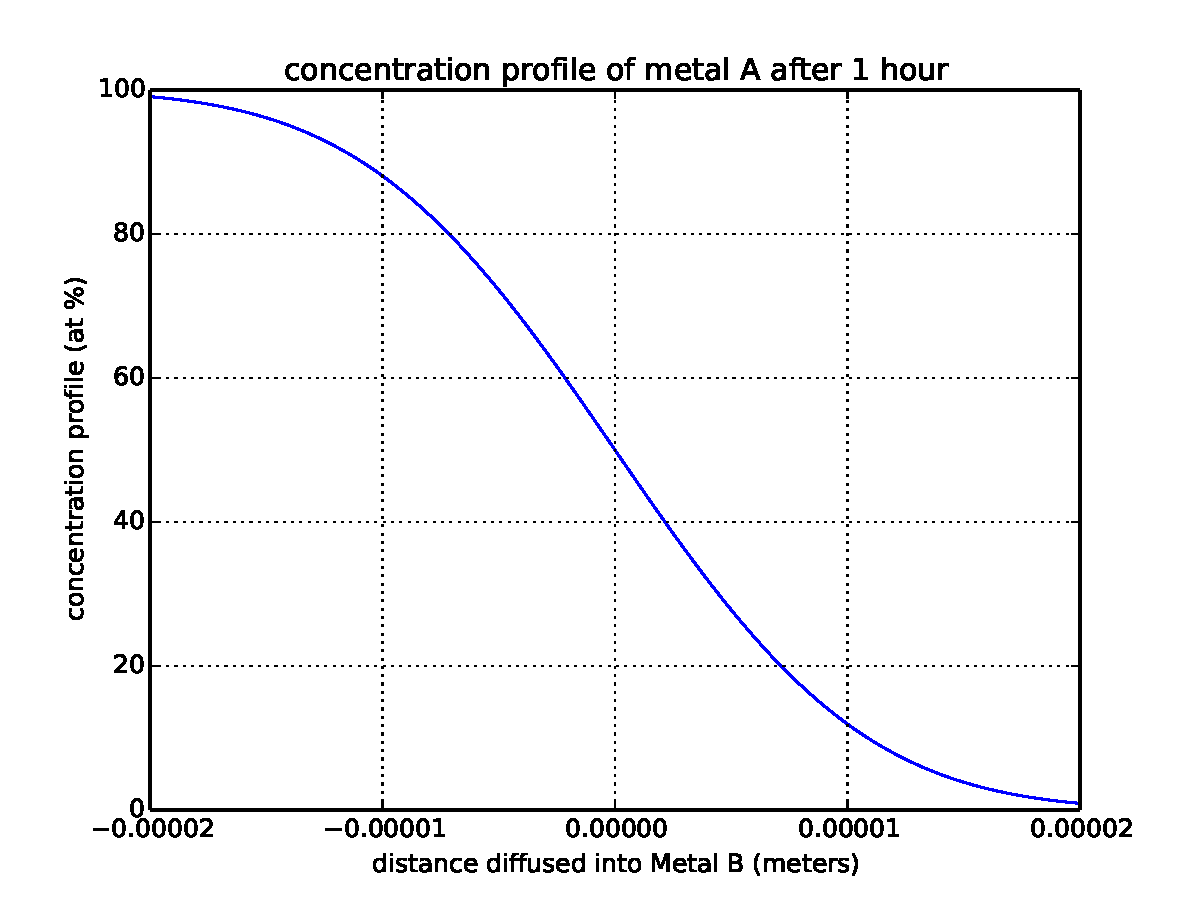
\includegraphics[width=350pt]{p2_graph.pdf}
\end{figure}

\begin{problem}{5.14}
Using the results of Problem \textbf{5.12} and assuming that profile occurred at a temperature of 1,000$\degree$C, superimpose the concentration profile of metal A for the same diffusion couple for 1 hour but heated at 1,200$\degree$C at which D = $\ex{-13} \,m^2/s$.
\end{problem}

\begin{figure}[H]
\centering
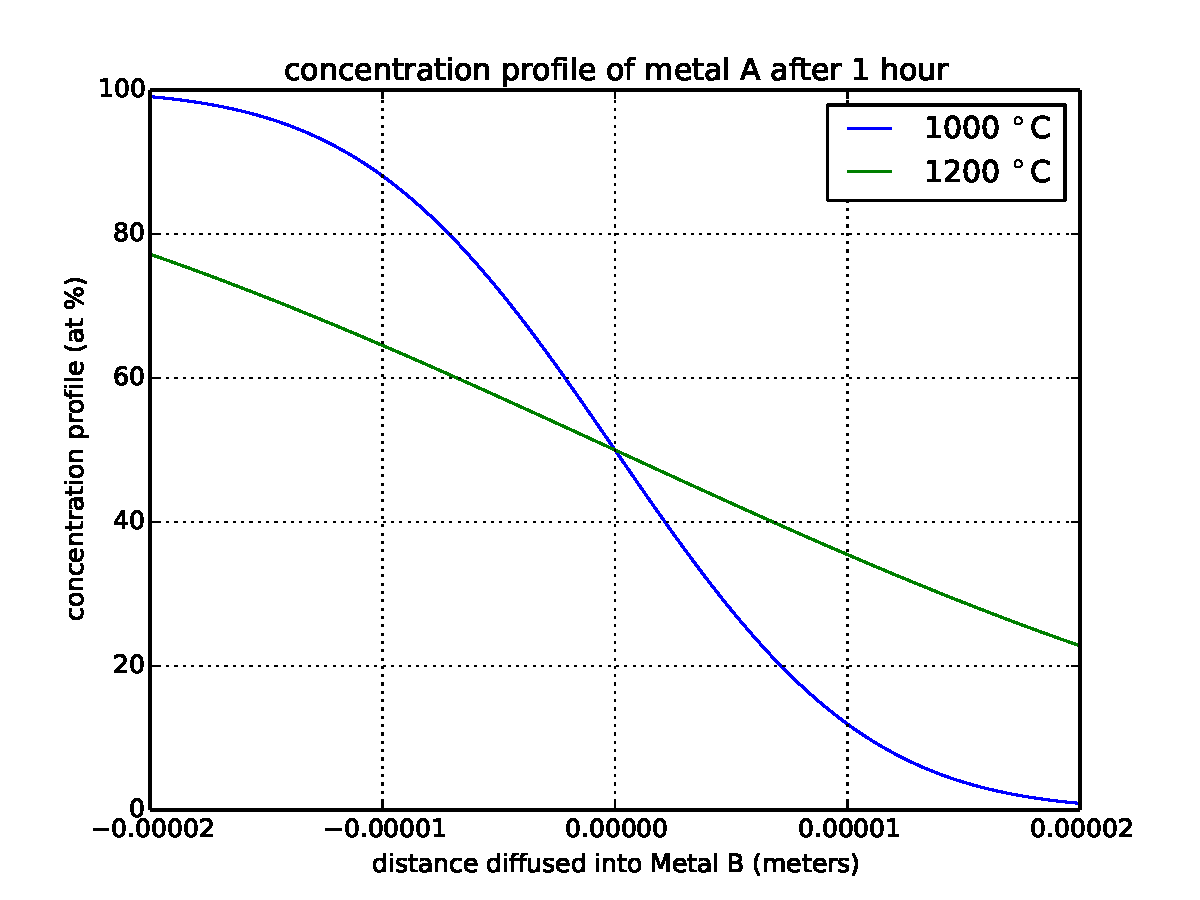
\includegraphics[width=350pt]{p3_graph.pdf}
\end{figure}

\begin{problem}{5.24}
Diffusion length, $\lambda$, is a popular term in characterizing the production of semiconductors by the controlled diffusion of impurities into a high-purity material.  The value of $\lambda$ is taken as $2\sqrt{Dt}$, where $\lambda$ represents the extent of diffusion for an impurity with a diffusion coefficient, D, over a period of time, t.  Calculate the diffusion length of B in Ge for a total diffusion time of 30 minutes at a temperature of \textbf{(a)} 800$\degree$C and \textbf{(b)} 900$\degree$C.  
\end{problem}

Using the data from Table 5.3 on page 139 of Shackelford [1] we see that for B Ge $D_0 = 1.1 \e{3} m^2/s$ and $Q = 439kJ/mol$.
\begin{equation}
D = D_0 \mathrm{e}^{\frac{-Q}{RT}}
\end{equation}
where $D_0$ is the preexponential constant, $Q$ is the activation energy, $R$ is the gas constant, and $T$ is temperature

\textbf{(a)}
\begin{align*}
\lambda = \sqrt{Dt} = \sqrt{D_0 \mathrm{e}^{\frac{-Q}{RT}}t} = \sqrt{1.1\e{3}m^2/s \,\mathrm{e}^{\frac{-439000J}{(8.314)(800 + 273.15)K}}*1800s} = 29.1 \,\text{nm}
\end{align*}

\textbf{(b)}
\begin{align*}
\lambda = \sqrt{Dt} = \sqrt{D_0 \mathrm{e}^{\frac{-Q}{RT}}t} = \sqrt{1.1\e{3}m^2/s \,\mathrm{e}^{\frac{-439000J}{(8.314)(900 + 273.15)K}}*1800s} = 238 \,\text{nm}
\end{align*}

\begin{problem}{5.29}
The endpoints of the Arrhenius plot of $D_{\text{grain boundary}}$ in Figure 5.18 are $D_{\text{grain boundary}} = 3.2\e{-12} m^2/s$ at a temperature of $457\degree C$ and $D_{\text{grain boundary}} = 1.0\e{-10} m^2/s$ at a temperature of $689\degree C$.  Using these data, calculate the activation energy for grain boundary diffusion is silver.
\end{problem}

\begin{equation}
D_2 = D_0 \mathrm{e}^{\frac{-Q}{RT_2}}
\end{equation}
\begin{equation}
D_1 = D_0 \mathrm{e}^{\frac{-Q}{RT_1}}
\end{equation}

Where $D_2 = 3.2\e{-12}m^2/s$, $D_1 = 1.0\e{-10}m^2/s$, $T_2 = 730.15 K$, and $T_1 = 962.15$.

Divide equation 3 by equation 4

\begin{align*}
\frac{D_2 = D_0 \mathrm{e}^{\frac{-Q}{RT_2}}}{D_1 = D_0 \mathrm{e}^{\frac{-Q}{RT_1}}} \Rightarrow \frac{D_2}{D_1} = \frac{\mathrm{e}^{\frac{Q}{RT_1}}}{\mathrm{e}^{\frac{Q}{RT_2}}} \Rightarrow \frac{D_2}{D_1} = \mathrm{e}^{\frac{Q}{R}(\frac{1}{T_1} - \frac{1}{T_2})} \Rightarrow \mathrm{ln}(\frac{D_2}{D_1}) = \mathrm{ln}(\mathrm{e}^{\frac{Q}{R}(\frac{1}{T_1} - \frac{1}{T_2})}) \\*[1cm]
 \mathrm{ln}(\frac{D_2}{D_1}) = \frac{Q}{R}(\frac{1}{T_1} - \frac{1}{T_2}) \Rightarrow Q = \frac{RT_2T_1\mathrm{ln}(\frac{D_2}{D_1})}{T_1 - T_2} = \frac{8.315*730.15K*962.15\mathrm{ln}(\frac{3.2\e{-12}}{1.0\e{-10}})}{962.15 - 730.15} \\*[1cm] Q = -86664.74\,\text{Joules/mole} = -86.7\,\text{kJ/mole}
\end{align*}


\section{References}
\begin{enumerate}
\item James F. Shackelford, Introduction to Materials Science for Engineers, Seventh Edition, Pearson Higher 
Education, Inc., Upper Saddle River, New Jersey (2009).
\end{enumerate}




% --------------------------------------------------------------
%     You don't have to mess with anything below this line.
% --------------------------------------------------------------
 
\end{document}
